\documentclass[tikz,border=8pt]{standalone}
\usepackage{amsmath}
\usetikzlibrary{arrows.meta}
\begin{document}
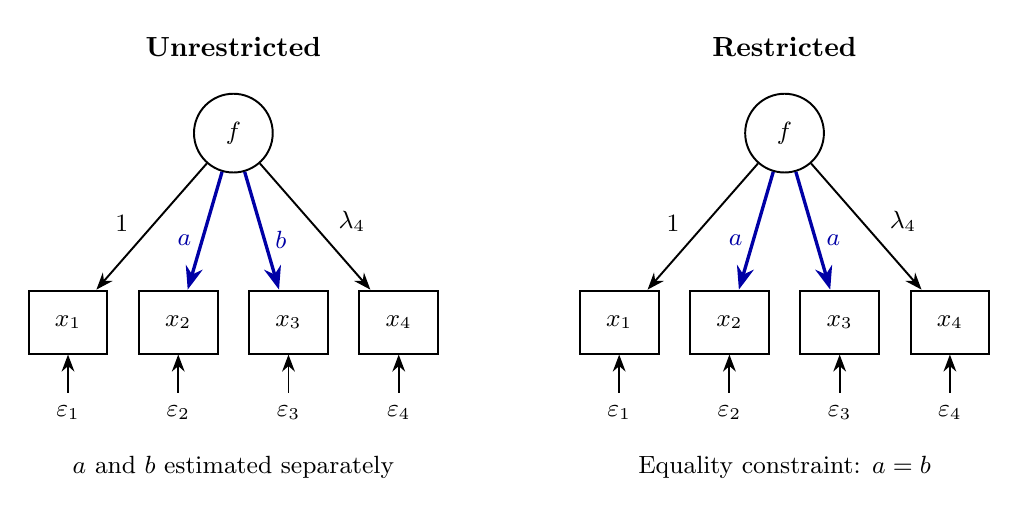
\begin{tikzpicture}[>=Stealth, line width=.7pt,
 observed/.style={draw,rectangle,minimum width=10mm,minimum height=8mm},
 latent/.style={draw,circle,minimum size=10mm},
 focus/.style={draw=blue!65!black,line width=1.2pt},
 every node/.style={font=\small}]
\foreach \shift/\heading/\alabel/\blabel in {0/Unrestricted/a/b,7/Restricted/a/a} {
 \begin{scope}[xshift=\shift cm]
 \node[font=\bfseries] at (0,3.5) {\heading};
 \node[latent] (f) at (0,2.4) {$f$};
 \foreach \i/\x in {1/-2.1,2/-.7,3/.7,4/2.1} {
  \node[observed] (x\i) at (\x,0) {$x_{\i}$};
  \draw[->] (\x,-.9) -- (x\i);
  \node at (\x,-1.15) {$\varepsilon_{\i}$};
 }
 \draw[->] (f) -- node[pos=.62,above left] {$1$} (x1);
 \draw[->,focus] (f) -- node[pos=.58,left,text=blue!65!black] {$\alabel$} (x2);
 \draw[->,focus] (f) -- node[pos=.58,right,text=blue!65!black] {$\blabel$} (x3);
 \draw[->] (f) -- node[pos=.62,above right] {$\lambda_4$} (x4);
 \end{scope}
}
\node at (0,-1.85) {$a$ and $b$ estimated separately};
\node at (7,-1.85) {Equality constraint: $a=b$};
\end{tikzpicture}
\end{document}
